% Created by tikzDevice version 0.12.3.2 on 2022-02-09 23:00:18
% !TEX encoding = UTF-8 Unicode
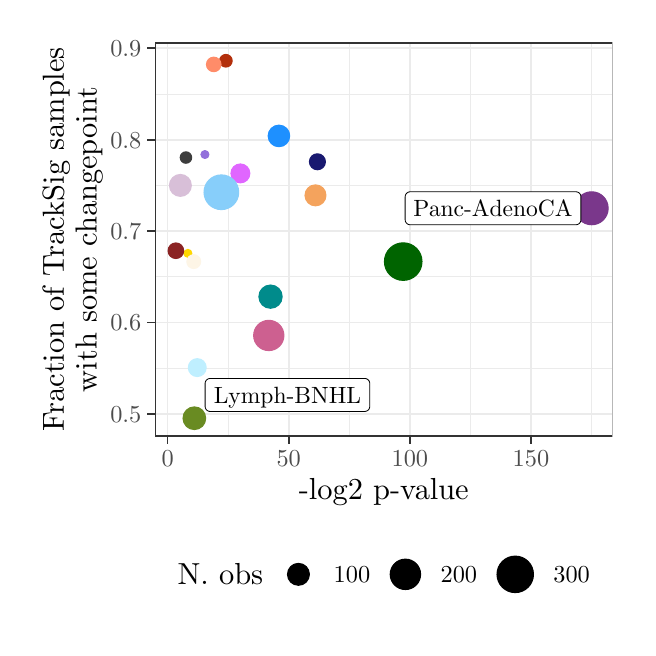
\begin{tikzpicture}[x=1pt,y=1pt]
\definecolor{fillColor}{RGB}{255,255,255}
\path[use as bounding box,fill=fillColor,fill opacity=0.00] (0,0) rectangle (216.81,216.81);
\begin{scope}
\path[clip] (  0.00,  0.00) rectangle (216.81,216.81);
\definecolor{drawColor}{RGB}{255,255,255}
\definecolor{fillColor}{RGB}{255,255,255}

\path[draw=drawColor,line width= 0.6pt,line join=round,line cap=round,fill=fillColor] (  0.00,  0.00) rectangle (216.81,216.81);
\end{scope}
\begin{scope}
\path[clip] ( 46.04, 69.22) rectangle (211.31,211.31);
\definecolor{fillColor}{RGB}{255,255,255}

\path[fill=fillColor] ( 46.04, 69.22) rectangle (211.31,211.31);
\definecolor{drawColor}{gray}{0.92}

\path[draw=drawColor,line width= 0.3pt,line join=round] ( 46.04, 93.74) --
	(211.31, 93.74);

\path[draw=drawColor,line width= 0.3pt,line join=round] ( 46.04,126.77) --
	(211.31,126.77);

\path[draw=drawColor,line width= 0.3pt,line join=round] ( 46.04,159.81) --
	(211.31,159.81);

\path[draw=drawColor,line width= 0.3pt,line join=round] ( 46.04,192.84) --
	(211.31,192.84);

\path[draw=drawColor,line width= 0.3pt,line join=round] ( 72.44, 69.22) --
	( 72.44,211.31);

\path[draw=drawColor,line width= 0.3pt,line join=round] (116.21, 69.22) --
	(116.21,211.31);

\path[draw=drawColor,line width= 0.3pt,line join=round] (159.98, 69.22) --
	(159.98,211.31);

\path[draw=drawColor,line width= 0.3pt,line join=round] (203.75, 69.22) --
	(203.75,211.31);

\path[draw=drawColor,line width= 0.6pt,line join=round] ( 46.04, 77.22) --
	(211.31, 77.22);

\path[draw=drawColor,line width= 0.6pt,line join=round] ( 46.04,110.26) --
	(211.31,110.26);

\path[draw=drawColor,line width= 0.6pt,line join=round] ( 46.04,143.29) --
	(211.31,143.29);

\path[draw=drawColor,line width= 0.6pt,line join=round] ( 46.04,176.32) --
	(211.31,176.32);

\path[draw=drawColor,line width= 0.6pt,line join=round] ( 46.04,209.36) --
	(211.31,209.36);

\path[draw=drawColor,line width= 0.6pt,line join=round] ( 50.56, 69.22) --
	( 50.56,211.31);

\path[draw=drawColor,line width= 0.6pt,line join=round] ( 94.33, 69.22) --
	( 94.33,211.31);

\path[draw=drawColor,line width= 0.6pt,line join=round] (138.10, 69.22) --
	(138.10,211.31);

\path[draw=drawColor,line width= 0.6pt,line join=round] (181.87, 69.22) --
	(181.87,211.31);
\definecolor{drawColor}{RGB}{255,215,0}
\definecolor{fillColor}{RGB}{255,215,0}

\path[draw=drawColor,line width= 0.4pt,line join=round,line cap=round,fill=fillColor] ( 57.90,135.25) circle (  1.43);
\definecolor{drawColor}{RGB}{205,96,144}
\definecolor{fillColor}{RGB}{205,96,144}

\path[draw=drawColor,line width= 0.4pt,line join=round,line cap=round,fill=fillColor] ( 87.12,105.59) circle (  5.46);
\definecolor{drawColor}{gray}{0.24}
\definecolor{fillColor}{gray}{0.24}

\path[draw=drawColor,line width= 0.4pt,line join=round,line cap=round,fill=fillColor] ( 57.19,169.88) circle (  2.06);
\definecolor{drawColor}{RGB}{216,191,216}
\definecolor{fillColor}{RGB}{216,191,216}

\path[draw=drawColor,line width= 0.4pt,line join=round,line cap=round,fill=fillColor] ( 55.18,159.81) circle (  3.95);
\definecolor{drawColor}{RGB}{25,25,112}
\definecolor{fillColor}{RGB}{25,25,112}

\path[draw=drawColor,line width= 0.4pt,line join=round,line cap=round,fill=fillColor] (104.70,168.35) circle (  2.88);
\definecolor{drawColor}{RGB}{30,144,255}
\definecolor{fillColor}{RGB}{30,144,255}

\path[draw=drawColor,line width= 0.4pt,line join=round,line cap=round,fill=fillColor] ( 90.79,177.69) circle (  3.89);
\definecolor{drawColor}{RGB}{139,35,35}
\definecolor{fillColor}{RGB}{139,35,35}

\path[draw=drawColor,line width= 0.4pt,line join=round,line cap=round,fill=fillColor] ( 53.55,136.21) circle (  2.81);
\definecolor{drawColor}{RGB}{179,47,11}
\definecolor{fillColor}{RGB}{179,47,11}

\path[draw=drawColor,line width= 0.4pt,line join=round,line cap=round,fill=fillColor] ( 71.62,204.85) circle (  2.27);
\definecolor{drawColor}{RGB}{0,100,0}
\definecolor{fillColor}{RGB}{0,100,0}

\path[draw=drawColor,line width= 0.4pt,line join=round,line cap=round,fill=fillColor] (135.70,132.28) circle (  6.78);
\definecolor{drawColor}{RGB}{253,245,230}
\definecolor{fillColor}{RGB}{253,245,230}

\path[draw=drawColor,line width= 0.4pt,line join=round,line cap=round,fill=fillColor] ( 60.00,132.28) circle (  2.48);
\definecolor{drawColor}{RGB}{105,139,34}
\definecolor{fillColor}{RGB}{105,139,34}

\path[draw=drawColor,line width= 0.4pt,line join=round,line cap=round,fill=fillColor] ( 60.23, 75.68) circle (  4.09);
\definecolor{drawColor}{RGB}{244,163,93}
\definecolor{fillColor}{RGB}{244,163,93}

\path[draw=drawColor,line width= 0.4pt,line join=round,line cap=round,fill=fillColor] (104.00,156.22) circle (  3.78);
\definecolor{drawColor}{RGB}{0,139,139}
\definecolor{fillColor}{RGB}{0,139,139}

\path[draw=drawColor,line width= 0.4pt,line join=round,line cap=round,fill=fillColor] ( 87.75,119.61) circle (  4.20);
\definecolor{drawColor}{RGB}{122,55,139}
\definecolor{fillColor}{RGB}{122,55,139}

\path[draw=drawColor,line width= 0.4pt,line join=round,line cap=round,fill=fillColor] (203.80,151.55) circle (  5.95);
\definecolor{drawColor}{RGB}{224,102,255}
\definecolor{fillColor}{RGB}{224,102,255}

\path[draw=drawColor,line width= 0.4pt,line join=round,line cap=round,fill=fillColor] ( 76.86,164.15) circle (  3.41);
\definecolor{drawColor}{RGB}{135,206,250}
\definecolor{fillColor}{RGB}{135,206,250}

\path[draw=drawColor,line width= 0.4pt,line join=round,line cap=round,fill=fillColor] ( 69.99,157.34) circle (  6.26);
\definecolor{drawColor}{RGB}{191,239,255}
\definecolor{fillColor}{RGB}{191,239,255}

\path[draw=drawColor,line width= 0.4pt,line join=round,line cap=round,fill=fillColor] ( 61.28, 93.98) circle (  3.22);
\definecolor{drawColor}{RGB}{147,112,219}
\definecolor{fillColor}{RGB}{147,112,219}

\path[draw=drawColor,line width= 0.4pt,line join=round,line cap=round,fill=fillColor] ( 64.05,170.97) circle (  1.43);
\definecolor{drawColor}{RGB}{255,140,105}
\definecolor{fillColor}{RGB}{255,140,105}

\path[draw=drawColor,line width= 0.4pt,line join=round,line cap=round,fill=fillColor] ( 67.23,203.53) circle (  2.62);
\end{scope}
\begin{scope}
\path[clip] ( 46.04, 69.22) rectangle (211.31,211.31);
\definecolor{drawColor}{RGB}{0,0,0}
\definecolor{fillColor}{RGB}{255,255,255}

\path[draw=drawColor,line width= 0.3pt,line join=round,line cap=round,fill=fillColor] ( 65.94, 78.14) --
	(121.80, 78.14) --
	(121.73, 78.14) --
	(122.02, 78.15) --
	(122.30, 78.21) --
	(122.58, 78.31) --
	(122.83, 78.46) --
	(123.05, 78.64) --
	(123.25, 78.86) --
	(123.40, 79.10) --
	(123.51, 79.37) --
	(123.58, 79.65) --
	(123.61, 79.94) --
	(123.61, 79.94) --
	(123.61, 88.23) --
	(123.61, 88.23) --
	(123.58, 88.52) --
	(123.51, 88.80) --
	(123.40, 89.07) --
	(123.25, 89.32) --
	(123.05, 89.53) --
	(122.83, 89.72) --
	(122.58, 89.86) --
	(122.30, 89.97) --
	(122.02, 90.02) --
	(121.80, 90.04) --
	( 65.94, 90.04) --
	( 66.15, 90.02) --
	( 65.86, 90.04) --
	( 65.57, 90.00) --
	( 65.30, 89.92) --
	( 65.03, 89.79) --
	( 64.79, 89.63) --
	( 64.58, 89.43) --
	( 64.41, 89.20) --
	( 64.27, 88.94) --
	( 64.18, 88.66) --
	( 64.13, 88.38) --
	( 64.13, 88.23) --
	( 64.13, 79.94) --
	( 64.13, 80.09) --
	( 64.13, 79.80) --
	( 64.18, 79.51) --
	( 64.27, 79.23) --
	( 64.41, 78.98) --
	( 64.58, 78.74) --
	( 64.79, 78.54) --
	( 65.03, 78.38) --
	( 65.30, 78.25) --
	( 65.57, 78.17) --
	( 65.86, 78.14) --
	cycle;
\end{scope}
\begin{scope}
\path[clip] ( 46.04, 69.22) rectangle (211.31,211.31);
\definecolor{drawColor}{RGB}{0,0,0}

\node[text=drawColor,anchor=base,inner sep=0pt, outer sep=0pt, scale=  0.85] at ( 93.87, 81.15) {Lymph-BNHL};
\definecolor{fillColor}{RGB}{255,255,255}

\path[draw=drawColor,line width= 0.3pt,line join=round,line cap=round,fill=fillColor] (138.21,145.60) --
	(198.11,145.60) --
	(198.03,145.60) --
	(198.32,145.61) --
	(198.61,145.67) --
	(198.88,145.77) --
	(199.13,145.92) --
	(199.36,146.10) --
	(199.55,146.32) --
	(199.71,146.56) --
	(199.82,146.83) --
	(199.89,147.11) --
	(199.91,147.40) --
	(199.91,147.40) --
	(199.91,155.69) --
	(199.91,155.69) --
	(199.89,155.98) --
	(199.82,156.26) --
	(199.71,156.53) --
	(199.55,156.78) --
	(199.36,157.00) --
	(199.13,157.18) --
	(198.88,157.32) --
	(198.61,157.43) --
	(198.32,157.49) --
	(198.11,157.50) --
	(138.21,157.50) --
	(138.43,157.49) --
	(138.14,157.50) --
	(137.85,157.46) --
	(137.57,157.38) --
	(137.31,157.26) --
	(137.07,157.09) --
	(136.86,156.89) --
	(136.68,156.66) --
	(136.55,156.40) --
	(136.46,156.12) --
	(136.41,155.84) --
	(136.40,155.69) --
	(136.40,147.40) --
	(136.41,147.55) --
	(136.41,147.26) --
	(136.46,146.97) --
	(136.55,146.70) --
	(136.68,146.44) --
	(136.86,146.21) --
	(137.07,146.00) --
	(137.31,145.84) --
	(137.57,145.72) --
	(137.85,145.63) --
	(138.14,145.60) --
	cycle;
\end{scope}
\begin{scope}
\path[clip] ( 46.04, 69.22) rectangle (211.31,211.31);
\definecolor{drawColor}{RGB}{0,0,0}

\node[text=drawColor,anchor=base,inner sep=0pt, outer sep=0pt, scale=  0.85] at (168.16,148.61) {Panc-AdenoCA};
\definecolor{drawColor}{gray}{0.20}

\path[draw=drawColor,line width= 0.6pt,line join=round,line cap=round] ( 46.04, 69.22) rectangle (211.31,211.31);
\end{scope}
\begin{scope}
\path[clip] (  0.00,  0.00) rectangle (216.81,216.81);
\definecolor{drawColor}{gray}{0.30}

\node[text=drawColor,anchor=base east,inner sep=0pt, outer sep=0pt, scale=  0.88] at ( 41.09, 74.19) {0.5};

\node[text=drawColor,anchor=base east,inner sep=0pt, outer sep=0pt, scale=  0.88] at ( 41.09,107.23) {0.6};

\node[text=drawColor,anchor=base east,inner sep=0pt, outer sep=0pt, scale=  0.88] at ( 41.09,140.26) {0.7};

\node[text=drawColor,anchor=base east,inner sep=0pt, outer sep=0pt, scale=  0.88] at ( 41.09,173.29) {0.8};

\node[text=drawColor,anchor=base east,inner sep=0pt, outer sep=0pt, scale=  0.88] at ( 41.09,206.33) {0.9};
\end{scope}
\begin{scope}
\path[clip] (  0.00,  0.00) rectangle (216.81,216.81);
\definecolor{drawColor}{gray}{0.20}

\path[draw=drawColor,line width= 0.6pt,line join=round] ( 43.29, 77.22) --
	( 46.04, 77.22);

\path[draw=drawColor,line width= 0.6pt,line join=round] ( 43.29,110.26) --
	( 46.04,110.26);

\path[draw=drawColor,line width= 0.6pt,line join=round] ( 43.29,143.29) --
	( 46.04,143.29);

\path[draw=drawColor,line width= 0.6pt,line join=round] ( 43.29,176.32) --
	( 46.04,176.32);

\path[draw=drawColor,line width= 0.6pt,line join=round] ( 43.29,209.36) --
	( 46.04,209.36);
\end{scope}
\begin{scope}
\path[clip] (  0.00,  0.00) rectangle (216.81,216.81);
\definecolor{drawColor}{gray}{0.20}

\path[draw=drawColor,line width= 0.6pt,line join=round] ( 50.56, 66.47) --
	( 50.56, 69.22);

\path[draw=drawColor,line width= 0.6pt,line join=round] ( 94.33, 66.47) --
	( 94.33, 69.22);

\path[draw=drawColor,line width= 0.6pt,line join=round] (138.10, 66.47) --
	(138.10, 69.22);

\path[draw=drawColor,line width= 0.6pt,line join=round] (181.87, 66.47) --
	(181.87, 69.22);
\end{scope}
\begin{scope}
\path[clip] (  0.00,  0.00) rectangle (216.81,216.81);
\definecolor{drawColor}{gray}{0.30}

\node[text=drawColor,anchor=base,inner sep=0pt, outer sep=0pt, scale=  0.88] at ( 50.56, 58.21) {0};

\node[text=drawColor,anchor=base,inner sep=0pt, outer sep=0pt, scale=  0.88] at ( 94.33, 58.21) {50};

\node[text=drawColor,anchor=base,inner sep=0pt, outer sep=0pt, scale=  0.88] at (138.10, 58.21) {100};

\node[text=drawColor,anchor=base,inner sep=0pt, outer sep=0pt, scale=  0.88] at (181.87, 58.21) {150};
\end{scope}
\begin{scope}
\path[clip] (  0.00,  0.00) rectangle (216.81,216.81);
\definecolor{drawColor}{RGB}{0,0,0}

\node[text=drawColor,anchor=base,inner sep=0pt, outer sep=0pt, scale=  1.10] at (128.67, 46.17) {-log2 p-value};
\end{scope}
\begin{scope}
\path[clip] (  0.00,  0.00) rectangle (216.81,216.81);
\definecolor{drawColor}{RGB}{0,0,0}

\node[text=drawColor,rotate= 90.00,anchor=base,inner sep=0pt, outer sep=0pt, scale=  1.10] at ( 13.08,140.27) {Fraction of TrackSig samples};

\node[text=drawColor,rotate= 90.00,anchor=base,inner sep=0pt, outer sep=0pt, scale=  1.10] at ( 24.96,140.27) {with some changepoint};
\end{scope}
\begin{scope}
\path[clip] (  0.00,  0.00) rectangle (216.81,216.81);
\definecolor{fillColor}{RGB}{255,255,255}

\path[fill=fillColor] ( 48.70,  5.50) rectangle (208.65, 33.04);
\end{scope}
\begin{scope}
\path[clip] (  0.00,  0.00) rectangle (216.81,216.81);
\definecolor{drawColor}{RGB}{0,0,0}

\node[text=drawColor,anchor=base west,inner sep=0pt, outer sep=0pt, scale=  1.10] at ( 54.20, 15.48) {N. obs};
\end{scope}
\begin{scope}
\path[clip] (  0.00,  0.00) rectangle (216.81,216.81);
\definecolor{fillColor}{RGB}{255,255,255}

\path[fill=fillColor] ( 90.61, 11.00) rectangle (105.07, 27.54);
\end{scope}
\begin{scope}
\path[clip] (  0.00,  0.00) rectangle (216.81,216.81);
\definecolor{drawColor}{RGB}{0,0,0}
\definecolor{fillColor}{RGB}{0,0,0}

\path[draw=drawColor,line width= 0.4pt,line join=round,line cap=round,fill=fillColor] ( 97.84, 19.27) circle (  3.95);
\end{scope}
\begin{scope}
\path[clip] (  0.00,  0.00) rectangle (216.81,216.81);
\definecolor{fillColor}{RGB}{255,255,255}

\path[fill=fillColor] (129.26, 11.00) rectangle (143.72, 27.54);
\end{scope}
\begin{scope}
\path[clip] (  0.00,  0.00) rectangle (216.81,216.81);
\definecolor{drawColor}{RGB}{0,0,0}
\definecolor{fillColor}{RGB}{0,0,0}

\path[draw=drawColor,line width= 0.4pt,line join=round,line cap=round,fill=fillColor] (136.49, 19.27) circle (  5.48);
\end{scope}
\begin{scope}
\path[clip] (  0.00,  0.00) rectangle (216.81,216.81);
\definecolor{fillColor}{RGB}{255,255,255}

\path[fill=fillColor] (167.92, 11.00) rectangle (184.45, 27.54);
\end{scope}
\begin{scope}
\path[clip] (  0.00,  0.00) rectangle (216.81,216.81);
\definecolor{drawColor}{RGB}{0,0,0}
\definecolor{fillColor}{RGB}{0,0,0}

\path[draw=drawColor,line width= 0.4pt,line join=round,line cap=round,fill=fillColor] (176.18, 19.27) circle (  6.58);
\end{scope}
\begin{scope}
\path[clip] (  0.00,  0.00) rectangle (216.81,216.81);
\definecolor{drawColor}{RGB}{0,0,0}

\node[text=drawColor,anchor=base west,inner sep=0pt, outer sep=0pt, scale=  0.88] at (110.57, 16.24) {100};
\end{scope}
\begin{scope}
\path[clip] (  0.00,  0.00) rectangle (216.81,216.81);
\definecolor{drawColor}{RGB}{0,0,0}

\node[text=drawColor,anchor=base west,inner sep=0pt, outer sep=0pt, scale=  0.88] at (149.22, 16.24) {200};
\end{scope}
\begin{scope}
\path[clip] (  0.00,  0.00) rectangle (216.81,216.81);
\definecolor{drawColor}{RGB}{0,0,0}

\node[text=drawColor,anchor=base west,inner sep=0pt, outer sep=0pt, scale=  0.88] at (189.95, 16.24) {300};
\end{scope}
\end{tikzpicture}
